\chapter{Case studies}
\label{chap:case-studies}
This chapter illustrates two case studies developed on the DingNet simulator.

The case study in \cref{sec:case-staudyLoRa} shows the DingNet platform after its extension.
The main new features used are the application layer that enables the communication between LoRaWAN gateways and applications, the managing of the incoming messages mote-side, and the new type of sensor.  
To do so, a system that requires a bi-directional communication between the application and the motes, and with the application behaviour dependent on the payload of the motes packets is conceived.

The case study in \cref{sec:case-staudyAC} exploits all the new features added in the DingNet simulator.
It uses the integration for the execution of Protelis application over DingNet, and the new type of simulation (\textit{TimedRun}) in addition to the features already used in the previous case study.
% unire i due capitoli
% avere due macro sezioni -> uno per caso
% farlo vedere come lavoro progressivo
% come prima cosa si vuole mettere in opera la piattaforma dingnet estesa con i nuovi requisiti ecc, per esercitarli si è pensato ad un caso di studio pensato in questa maniera con blabla 
% il secondo case study invece esercita la piattaforma alla sua piena potenza quindi sfrutta il già testato ambaradm di dingnet esteso e la nuova integrazione di protelis su dingnet

\section{Case study: Pollution-aware user navigation}
\label{sec:case-staudyLoRa}

% This chapter presents the case study used as reference scenario during the evolution of the DingNet simulator, and to evaluate the limits of communications from applications to LoRa motes. 
% A demo from this case study was showed during the Day of Science in Flanders to present the LoRaWAN technology receiving a lot of attention.

% \section{Case study description}
Leuven is a cycling city where most of the inhabitants and students use daily their bike to move across the city. 
In this context we want to realise a system able to provide to the user the healthiest route to reach a destination. 
The route generation will be based on the air quality level, based on the CAQI index~\cite{CAQI}, of the crossed areas to reach the destination. 
The user, in order to obtain the route, has to require it to the application deployed in a remote server.
The system uses data received from the sensor network to create a city map of quality air.
Then, the application has to define the route to a destination that optimise the trade-off between air quality and length of the route.
The system should be able to recompute the best route if the environment condition change, and communicate it to the user.
The sensor network can be composed by two types of sensors:
\begin{itemize}
    \item \textbf{Fixed}: positioned along the roads and at intersections
    \item \textbf{Mobile}: placed on public transport or bicycles
\end{itemize}
All the sensors have to be deployed in a LoRaWan network.
Similarly also the user device, which interacts with the application to require the route, has to use the LoRa technology.

\subsection{Design of the system}
\autoref{fig:caseStudyA} shows the high level architecture of the system, and introduces the main entities. 
The main entities are the sensors devices, the user devices, and the routing application.
As requirement both sensors devices and user devices have to be displaced inside the LoRaWAN network and use the LoRa technology to communicate with the routing application.
Using the DingNet simulator to simulate the LoRaWAN network:
\begin{itemize}
    \item the routing application is mapped in a generic application deployed in the application server that communicates with the LoRaWAN network via MQTT
    \item the sensor devices, which have to send only packet with the sensed value, can be mapped in the \textit{Mote} simulator entity
    \item the user devices are special devices, because they do not send only packets with the sensed value. They have also to require the route for a destination and be able to manage the received packets with the route. Actually there is not simulator entity with this specific abilities, so it will be necessary to define it.
\end{itemize}
% 
\begin{figure}[h]
    \centering
    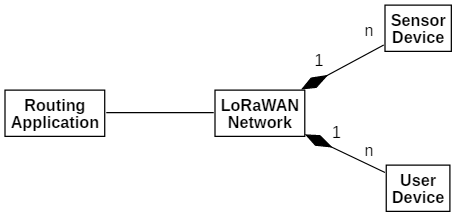
\includegraphics{figures/CaseStudyA_HLarch.png}
    \caption{High level architecture of the system}
    \label{fig:caseStudyA}
\end{figure}
% 

\subsection*{Interaction between application and devices}
If on one hand the transmissions from the devices (both sensor and user) to the application are in compliance with the maximum packet's length defined by the LoRaWAN standard (1 byte for packets with the sensed value, and 16 bytes for the packet to require the route); on the other hand it is impossible to send the packet from application to the user device with the entire route, so the only way to do it is to split the packet.
In order to send the entire route to the user device, two approaches are available: 
\begin{enumerate}
    \item define a specific interaction protocol to send all the packets with the entire route to the user device immediately after its computation
    \item send a packet with part of the route only when the user has finished the previous part of the route.
\end{enumerate}
Considering also the requirement to recompute the route if the environment condition change, the second option is chosen, enabling to recompute the route before send its next part.

\subsection*{User device model}
% UserMote - consume packet
The user device has to perform three activity: require the route, send update of its position, and manage the incoming packets.
If on one hand the last two activity can be performed also from a \textit{Mote}, on the other hand it cannot require the route.
For this reason in \autoref{fig:userMote} a new entity simulator is introduced, the \textit{UserMote}. 
It extends the \textit{Mote} adding the logic to require the route when needed sending a packet with starting and destination positions.
Then to manage incoming packets are chosen \textit{MaintainLastPacket} as strategy to store them until that they are consumed, and \textit{ReplacePath} as only strategy to consume them.
It consumes each packet updating the user route in accord with the packet payload until the route is completed.
To perform the last activity, send updating of the user position, is only necessary add the GPS sensor to the \textit{UserMote}, and send it when the user is closer to the sub-route destination.
% 
\begin{figure}[h]
    \centering
    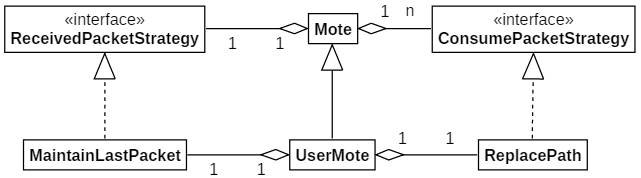
\includegraphics{figures/userMote.png}
    \caption{\textit{UserMote} model.}
    \label{fig:userMote}
\end{figure}
% 

\subsection*{Routing application}
The application to found the best route implements an A-star algorithm on the graph of street of the city. 
The weight of the edges of the graph corresponds to the distance between the two points multiply for a factor that represents the air quality level in that street. 
The values sensed by the sensors are retrieved subscribing the topics where the LoRaWAN network publishes them. 
The route is sent to the user mote publishing the massage with sub-route on its receiving topic.
The application recomputes the best route only when the user device communicates its new position and if some environment condition is changed from the previous computation.

\subsection{Simulation in DingNet}
Here, simulations of two possible small scale scenarios are illustrated. 
The simulations are conducted over the city of Leuven with the DingNet simulator.
First, the setup of the two simulated scenarios is presented; then the simulation results discussed in a qualitative way based on simulation snapshots.

\subsection*{Setup}
Both the scenarios present a common configuration and differ only for the starting position of the user.
The environment is composed of:
\begin{itemize}
    \item 2 gateways
    \item 4 fixed sensors equipped with a set of sensors and send directly the final CAQI index value.
    \item one mobile sensor that follows a path like a public transport. It assume the same behaviour of a fixed sensor, but is equipped also of a GPS sensors.
    \item user that requires a route to a destination.
\end{itemize} 
All the types of LoRa devices are configured in a way to try to reduce collision between transmissions.
In the first scenario the user start from the south of the city, which is the most polluted in the simulation configuration; while in the second scenario the user starts from the north of the city.

\subsection*{Results}

\autoref{fig:sim1} and \autoref{fig:sim2} show snapshots taken from the two simulated scenarios.
The transparent layer represents the air quality level in that point based on the received sensor value.
The mote number 4 is the mobile sensor and the red line is its route.
The user is identified by the cyclist. 
Its line (route) is of two colours: blue and red.
The blue one is the complete route computed by the application, while the red one is the sub-route received by the user until that time. 

\autoref{fig:sim1} shows three snapshots of the first simulated scenario.
The first snapshot shows the initial situation and the first computed route.
The second snapshot shows how after an environment conditions change, the route is recomputed with a longer one, but considered better by the application, combining distance with pollution. 
So the user has received a new sub-route of the new best route that starts from its actual position.
Finally, the last snapshot shows the user arrived to destination.
% 
\begin{figure}[h]
    \centering
    \begin{tabular}{lll}
         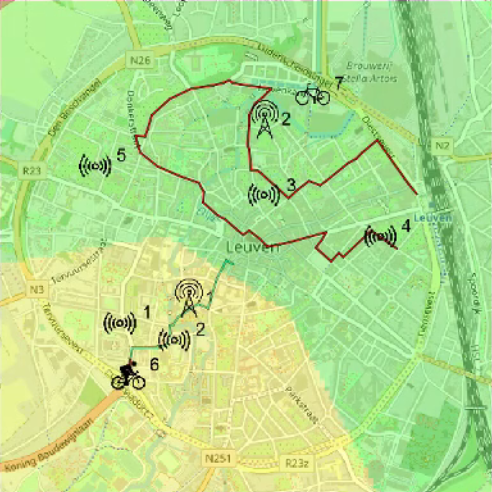
\includegraphics[scale=0.42]{figures/sim1snap1.png}  &
         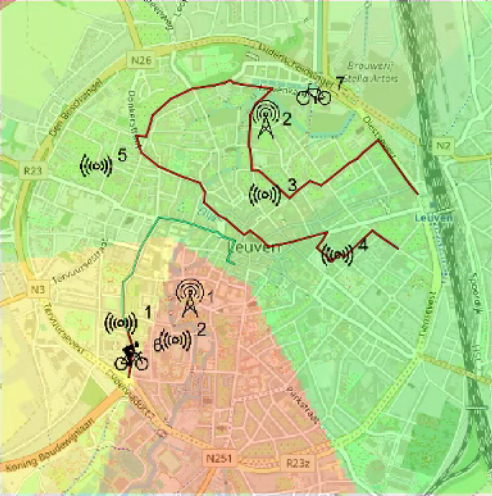
\includegraphics[scale=0.42]{figures/sim1snap2.png} &
         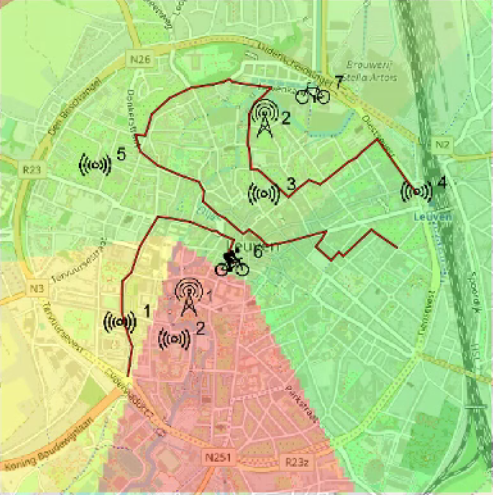
\includegraphics[scale=0.42]{figures/sim1snap3.png} 
    \end{tabular}
    \caption[Three snapshots of a simulation run with changing of the route]{Three snapshots of a simulation run with changing of the route dues to the change of the environment conditions.}
    \label{fig:sim1}
\end{figure}
% 

\noindent \autoref{fig:sim2} shows three snapshots of the second simulated scenario.
In this case the user best route never changes because the change of the environmental conditions do not affect the areas crossed by him.
% 
\begin{figure}[h]
    \centering
    \begin{tabular}{lll}
         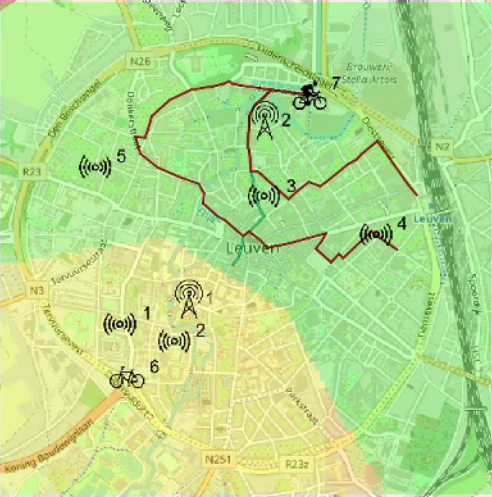
\includegraphics[scale=0.42]{figures/sim2snap1.png}  &
         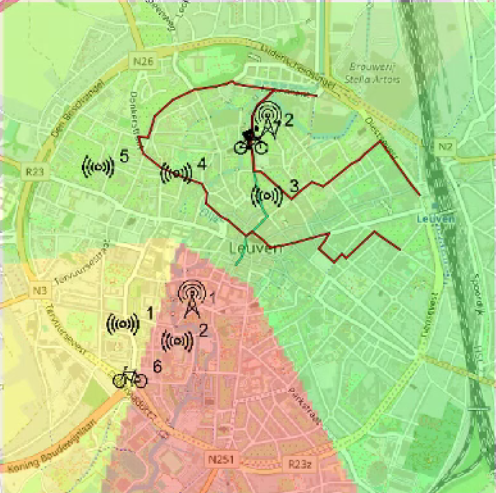
\includegraphics[scale=0.42]{figures/sim2snap2.png} &
         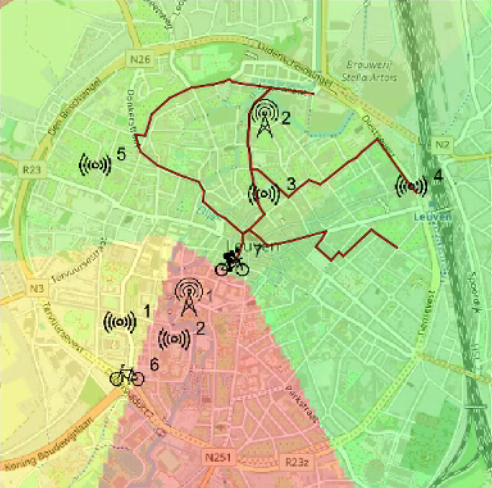
\includegraphics[scale=0.42]{figures/sim2snap3.png} 
    \end{tabular}
    \caption[Three snapshots of a simulation run without changing of the route]{Three snapshots of a simulation run without changing of the route despite the change of the environmental conditions.}
    \label{fig:sim2}
\end{figure}
% 

Although they are simple simulations with few sensors and only one user device, it can be deduced that use LoRa technology also for user devices is possible only in certain scenarios.
In these scenarios the number of transmissions necessary to transmit all the route is high, so according to LoRaWAN limitations it is possible only for short route.
Moreover considering a real scenario where the number of user is higher (es. more than one thousand) the network congestion will increase with also the probability of collisions among transmissions, which require re-transmission worsening the situation.
\section{Case study: Monitoring and control of air quality}

\label{sec:case-staudyAC}
% This chapter presents a case study that joins the aggregate computing paradigm and a LoRaWAN network. Finally, it shows a simulation of the case study in the DingNet simulator.

Nowadays air pollution is a very common problem of cities of all the world.
Two of the main strategies used to reduce the emission of polluting gas are traffic bans in strategic city's areas, and maximum temperature allowed in public and private building heating.

In this context we want to realise a monitoring system for the air quality based on the CAQI index~\cite{CAQI}, which is able to apply strategies to maintain under control the air pollution level.
The sensor network is composed of a set of fixed sensors scattered around the city, and mobile sensors placed on public transports (like bus or public bicycles).
All the sensor devices are equipped at least with a sensor for the particular matter 10 (PM10).
The idea is to displace strategically the fixed sensors to achieve a good city coverage, using mobile sensors for its refinement and to reduce reading errors of the fixed ones.

In a first step to reduce air pollution it has been chosen to control the maximum temperature allowed for the heating of buildings.
The idea is to allow the system to manage the building heating systems control devices (from now on building devices). So the system can set the maximum reachable temperature based on pollution level of its area.

All the sensors have to be displaced in a LoRaWAN network to communicate their sensed data to reduce their cost and the cost for their maintenance. 
Building devices have not any particular requirements, they have not problems of energy consumption because they can be connected to the power line of the building.
The same policy can be adopted for the Internet connection, this allows to avoid to use LoRa technology reducing the number of LoRa devices in the network and increasing their communication capability.

\subsection{Design of the system}

Aggregate computing is a good approach for this system for several reasons.
First of all, it is a heterogeneous system composed for at least two types of devices (sensor and building device) with different capabilities like connectivity, computational resources, and their interaction with the environment. 
Furthermore it is composed from an high number of devices (one device building for each house of the city, a set of fixed sensors, and a set of mobile ones) so scalability can be a problem. But with aggregate computing is possible to solve it scaling horizontally and moving the computational node in different network devices without the need to change the program.
\autoref{fig:caseStudyAC} shows a high level architecture of the system.
\begin{figure}[h]
    \centering
    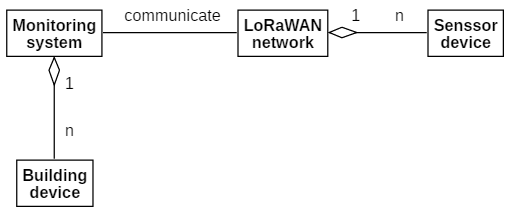
\includegraphics{figures/caseStudyB_high.png}
    \caption{High level architecture of the system}
    \label{fig:caseStudyAC}
\end{figure}
\\Designing the system with the aggregate computing is important to model the two different kind of devices and the communication layer of the aggregate nodes.

\subsection*{Sensors and building devices models}
The sensor devices are LoRa motes, so they are mapped in \mbox{\textit{Mote}} inside DingNet, while, according to \cref{sec:PoverD}, in the aggregate application they can be mapped in simple \mbox{\textit{ProtelisLoRaNode}}.
The building devices are not LoRa motes, so they do not require to be mapped in \mbox{\textit{ProtelisLoRaNode}} and they can be generic Protelis nodes.
Anyway it is decided to map them in \mbox{\textit{BuildingNode}}, which extends \mbox{\textit{ProtelisLoRaNode}}, \autoref{fig:caseBmodel_a}. This because:
\begin{itemize}
    \item the building node has not a physical mote then its topic will never receive a MQTT message, so it has not any overhead;
    \item all the types of nodes have a base \mbox{\textit{ExecutionContext}} where introduce functions domain specific;
    \item if in the future they will have a physical mote, it will not be necessary to change the system architecture.
\end{itemize}
\autoref{fig:caseBmodel_b} completes the model of the entities with their \mbox{\textit{ExecutionContext}}.
\mbox{\textit{SensorExecutionContext}} updates the knowledge-base of the node computing the CAQI index at each new sensed data received. It contains also all the methods for the logic domain specific. \mbox{\textit{BuildingExecutionContext}} extends it adding the capability to modify the temperature in its physical counterpart.
\begin{figure}[h]
    \centering
    \begin{subfigure}{.495\textwidth}
        \centering
        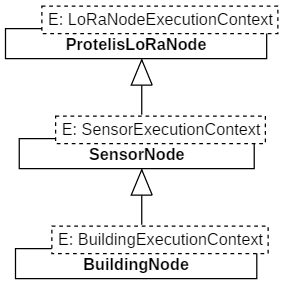
\includegraphics{figures/NodeAC_caseStudy.png}
        \caption{}
        \label{fig:caseBmodel_a}
    \end{subfigure}
    \begin{subfigure}{.495\textwidth}
        \centering
        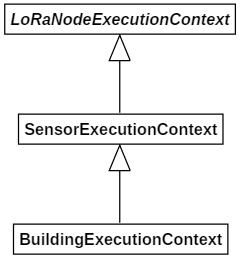
\includegraphics{figures/ECAC_caseStudy.png}
        \caption{}
        \label{fig:caseBmodel_b}
    \end{subfigure}
    \caption{Model of the aggregate entities.}
    \label{fig:caseBmodel}
\end{figure}

\subsection*{Interaction between Protelis nodes}
In order to complete the Protelis backend is required to implement the communication layer. It has to:
\begin{enumerate}
    \item define the neighbourhood policy to determine the neighbours of each node;
    \item design and implement the communication between the Protelis nodes.
\end{enumerate}
As neighbourhood policy a distance based one is chosen. 
This policy is chosen considering the application domain, in fact the behaviour of each node depends on the environment state in its area.\\ 
MQTT is chosen to implement the \mbox{\textit{NetworkManager}} and enable the communication between Protelis nodes.
MQTT is chosen because it is a lightweight protocol and enables devices to send the same message to more devices with only one communication.
This is very important in a large scale system where the nodes are displaced in many places and the connectivity can go down. \\
This system is composed also from mobile nodes and when one node change position its neighbours can change, as the neighbourhood of other nodes. 
So the definition of the neighbourhood cannot be done only at configuration time, but it has to performed also after.
The \mbox{\textit{NeighborhoodManager}} is an autonomous entity defined to manage the neighbourhood of all the nodes.
It receives the update of the node position, recomputes the neighbourhoods, and communicates their to all the nodes. 
This entity allows also to modify the composition of the system at run-time, adding or removing entities with all the neighbourhood updated automatically.

\subsection{Protelis program}
After discussing the design of the Protelis back-end, this section introduces the Protelis program for the global behaviour of the system. 
The program, visible in \autoref{lst:program}, requires only 25 lines of code.
Methods \mbox{\textit{decreaseTemp}} and \mbox{\textit{increaseTemp}} modify the temperature of the building devices of a delta temperature every half an hour.
These methods are build on top of the function \mbox{\textit{cyclicFunction}}, which is present in the developer API of the aggregate stack.
Lines 16 - 23 first create a computational field of sensed values and distances from the respective sensor. 
Then they manipulate it defining a field of maximum temperature allowed for each device based on CAQI index.
The final part of the program defines the target temperature for each device and selects the correct method to achieve it. 

\lstinputlisting[
	float,
	language=Protelis,
	caption={Protelis program for the monitoring application},
	label={lst:program},
]{listings/homeHeating_timer.pt}

\subsection{Simulation in DingNet}
Here, a simulation of a possible scenario is illustrated. 
The simulation is conducted over the city of Leuven with the DingNet simulator.
First, the setup of the simulated scenario is presented; then the simulation results are discussed in a qualitative way based on simulation snapshots.
% la valutazione è di tipo qualitativo per il momento, ma che ulteriori valutazioni di tipo quantitativo sono allo studio e materia di futara pubblicazione 
\subsection*{Setup}
The configuration of the simulation provides for an environment composed of the following entities:
\begin{itemize}
    \item 9 of the 11 DingNet network gateways (the others two are outside of the simulation region);
    \item 8 fixed sensors equipped with the PM10 sensor;
    \item 2 mobile sensors equipped with PM10 and GPS sensors;
    \item 3 building devices displaced in three different areas of the city.
\end{itemize}
All the sensors are configured to send a new measurement every hour, according to the CAQI index specifications for this polluting gas.
The low number of mobile sensors and building devices is only due to visualisation purposes. 

\subsection*{Results}
\autoref{fig:simAC} shows three snapshots taken from a simulation run of five days.
The transparent layer represents the air quality level, which is obtained applying an inverse distance weighting on sensed values in the range of 1Km. 
Green colour means ``very low'' level, while red colour means ``high'' level.
The two motes with a red line are the mobile sensors, while the others are the fixed ones.
The building devices are represented with a black dot and a text with pattern ``X/Y/Z''.
X is its current temperature, Y is its desired temperature, and Z 
% 
\begin{figure}[h]
    \centering
    \begin{tabular}{ll}
         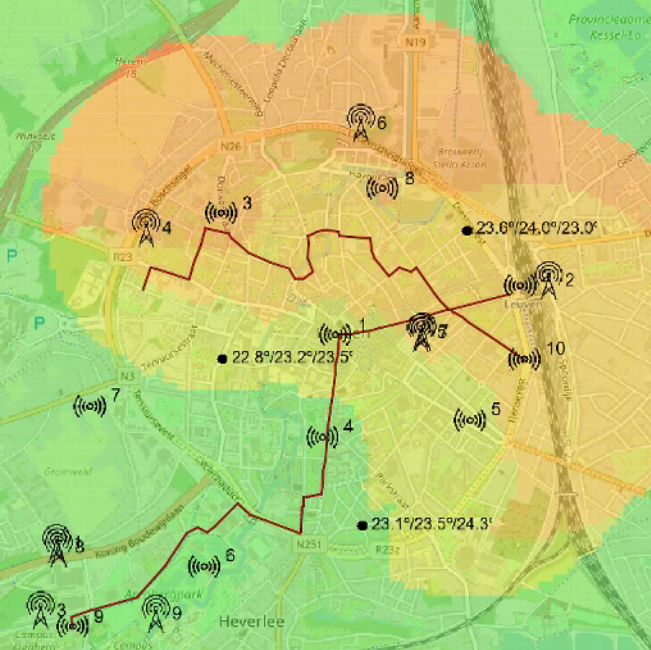
\includegraphics[scale=0.42]{figures/simACsnap1s.png}  &
         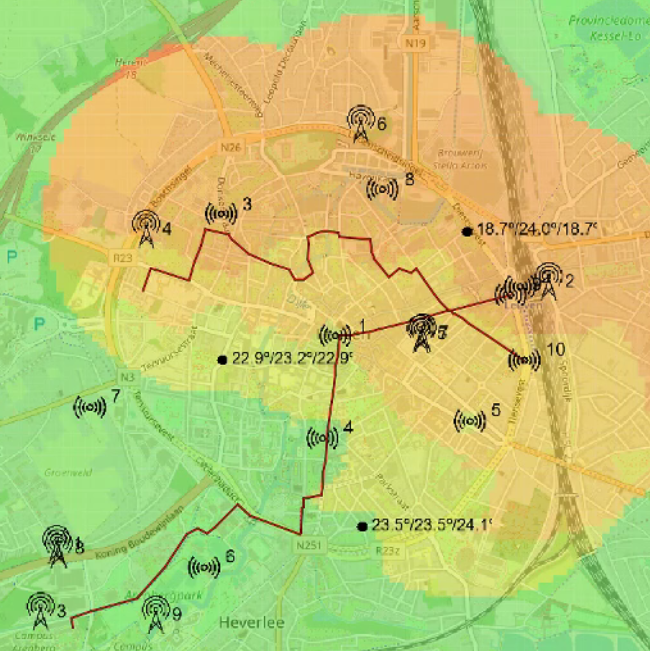
\includegraphics[scale=0.42]{figures/simACsnap2s.png}
    \end{tabular}
    \begin{tabular}{c}
         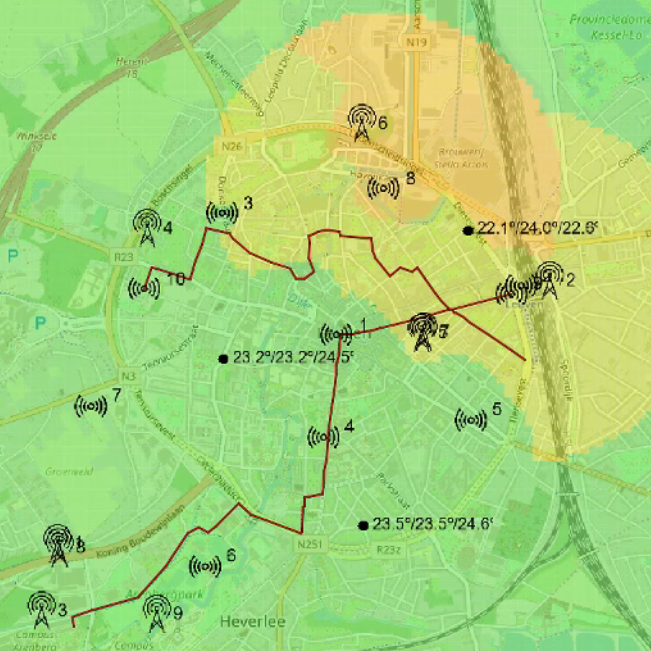
\includegraphics[scale=0.42]{figures/simACsnap3s.png} 
    \end{tabular}
    \caption[Snapshots of a simulation run (case study 2)]{Three snapshots of a simulation run.}
    \label{fig:simAC}
\end{figure}
% 
is its maximum reachable temperature based on pollution level.
The three snapshots show how the pollution changed during the five days of simulation, and how the building maximum reachable temperature is adapted consequently.
In particular the building in the north of the city has always the desired temperature greater then the maximum reachable. 
The building in the centre of the city has first the desired temperature greater then the maximum reachable, but after the pollution change it is the opposite and the building reaches its desired temperature.
Finally, the building in the south has always the desired temperature lower then the maximum reachable.





\paragraph{Concluding remarks.} This chapter illustrated two case-studies developed on the DingNet simulator.
The first one showed the new application layer of the simulator and the new main features. It confirmed the validity of LoRaWAN as enabling technology for a sensor network and its limits regarding the communication from application to LoRa devices.
The second case study showed an application developed using all the features of the platform and proved its validity as platform to simulate Protelis applications over a LoRaWAN network.

% This chapter has presented the case study used as reference for the simulator evolution. It has helped to consider the behaviour of all the network facilities and the bi-directional communication schema. It has confirmed the validity of LoRaWAN as enabling technology for a sensor network and its limits regarding the communication from application to LoRa devices.

% \paragraph{Concluding.} This chapter has presented a system designed with the aggregate computing paradigm over a LoRaWAN network, and simulated it in the DingNet simulator. After all the improvements and extensions on DingNet simulator, this case study has showed how it is possible simulate Protelis applications in this platform.